\subsection{Omnichain Engine}

The Omnichain Engine is a powerful interoperability framework built on the Hermes chain, with the Narada Service providing secure key management and execution support. Using the Tendermint consensus protocol for block creation, ensuring high-speed finality, Byzantine fault tolerance (BFT) and efficient transaction processing. Tendermint’s~\cite{tendermint} consensus mechanism is designed to provide fast block confirmation while maintaining security, making it ideal for cross-chain communication and decentralized execution.

At the core of the Omnichain Engine, the Hermes chain functions as the primary coordination layer, managing cross-chain transactions, state updates, and message passing between different rollups and blockchain networks. It ensure that cross-chain operations are executed efficiently and securely, serving as the backbone of the omnichain ecosystem.

\begin{figure}[h]
    \centering
    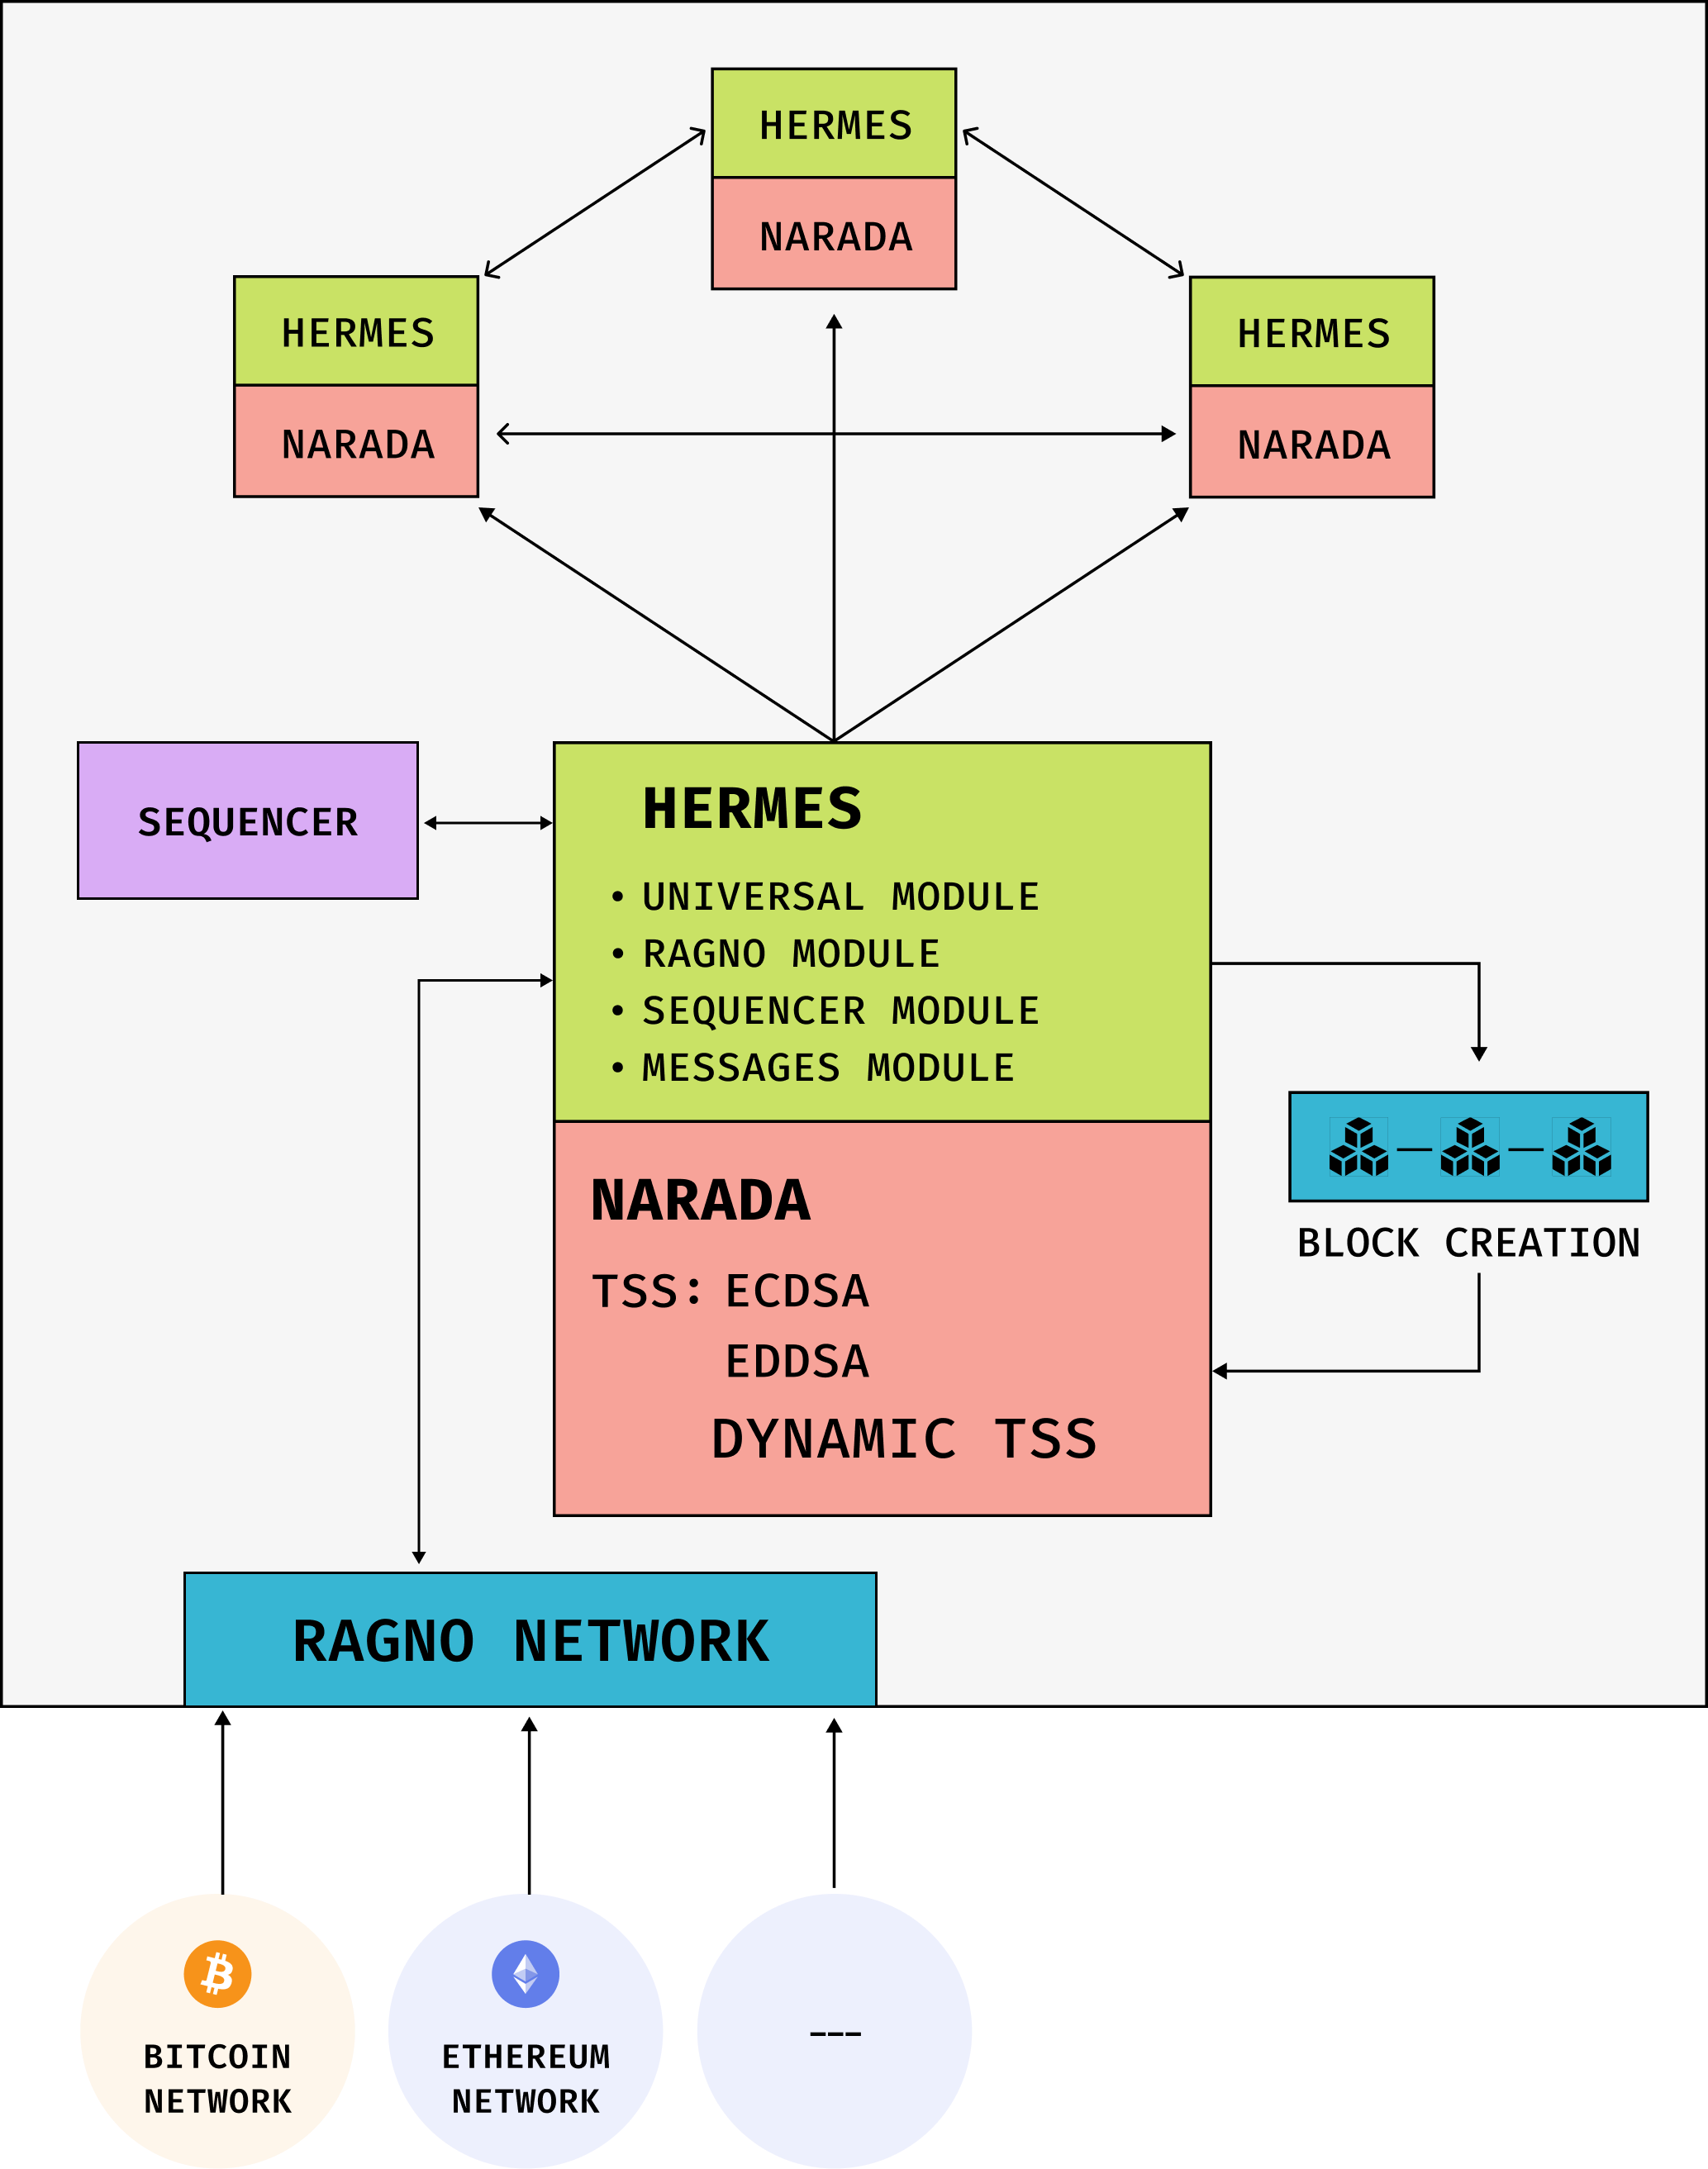
\includegraphics[width=0.7\linewidth]{figure/engine.png}
    \caption{Omnichain Egine}
    \label{fig:engine}
\end{figure}

A critical component of this architecture is the Narada Service, which provides the CGGMP Threshold Signature Scheme (TSS)~\cite{tss} functionality, enabling decentralized key management. This allows the Omnichain Engine to control and sign transactions for any addresses it manages without relying on a single point of failure. Furthermore, Narada extends TSS support to addresses controlled by private rollup clients, enabling enterprises and customized rollup solutions to securely manage cross-chain assets and operations.

By combining Tendermint’s fast and secure consensus, Hermes Chain’s interoperability capabilities, and Narada Service’s decentralized key management, the Omnichain Engine creates a trustless, scalable, and flexible environment for cross-chain transactions. This architecture empowers developers to build omnichain applications with seamless connectivity, robust security, and efficient execution.


\subsubsection{Threshold Signature Scheme (TSS)}

The cggmp TSS~\cite{tss} Scheme enables a distributed set of participants to collaboratively generate and use a cryptographic key for secure signing without having full control. The scheme consists of three key phases: \textsf{Key Generation}, \textsf{Pre-Signing}, and \textsf{Signing}, with an additional \textsf{Key Refresh} mechanism to maintain security over time.  

\begin{itemize}
    \item \textbf{Key Generation}
    
    Upon receiving the input (\textsf{keygen}, \textsf{sid}, $i$), the system initializes the key setup process:  
    \begin{itemize}
        \item[1.] Executes the key generation phase, obtaining the partial secret share $X_0$ and the public key $\textsf{pk}$.  
        \item[2.] Runs the auxiliary information phase, processing (\textsf{aux-info}, \textsf{sid}, $X_0$, $i$) to output essential parameters: $(\textsf{sid}, \textsf{rid}, X^*, N, s, t)$ and individual participant-specific values $(x_i, y_i, p_i, q_i)$.  Assigns an epoch identifier (\textsf{epid}) to encapsulate these parameters:  
     \[
     epid = (\textsf{sid}, \textsf{rid}, X^*, N, s, t)
     \]
        \item[3.] Outputs the public key $\textsf{pk}$ associated with the session identifier \textsf{sid}.  
    \end{itemize}

    \item \textbf{Pre-Signing} 
    
    To prepare for signing, the system processes the input $(\textsf{pre-sign}, \textsf{epid}, L, i)$:  
    \begin{itemize}
        \item[1.] Erases all previous presigning data associated with \textsf{epid} to maintain security.  
        \item[2.] Runs the pre-signing phase concurrently for all $l\in [L]$, initializing multiple pre-signing sessions.  
        \item[3.] Once presigning is completed, the system remains on standby, awaiting the actual signing request.  
    \end{itemize}

    \item \textbf{Signing}
    
    When a signature is requested for a message \textsf{msg}, the system processes $(\textsf{sign}, \textsf{epid}, \textsf{sgid}, l, i, \textsf{msg})$ as follows: 
    \begin{itemize}
        \item[1.] Converts the message \textsf{msg} into a standardized form $m = F(\textsf{msg})$.  
        \item[2.] Runs the signing phase with input $(\textsf{sign}, \textsf{epid}, \textsf{sgid}, l, i, m)$ to generate a signature $\sigma$ and a verification set $Q$:  If $\sigma$ is valid, $Q = \phi$. Otherwise, $Q$ contains the identifier of a detected corrupted party.  
        \item[3.] Outputs the signature tuple:  
   \[
   (\textsf{sig-string, sid, sgid, msg}, \sigma, Q)
   \]  
    \end{itemize}

    \item \textbf{Key Refresh}  
    
    To refresh cryptographic keys, the system processes $(\textsf{key-refresh, sid}, X, i)$, ensuring continued security and integrity.  
    \begin{itemize}
        \item[1.] Runs the auxiliary information phase on $(\textsf{aux-info, sid}, X, i)$.  
        \item[2.] Retrieves updated parameters $(\textsf{sid, rid}, i, X^*, N, s, t)$ along with participant-specific values $(x_i, y_i, p_i, q_i)$.  
        \item[3.] Erases all previous presigning and auxiliary information related to the prior \textsf{epid}.  
        \item[4.] Assigns a new \textsf{epid}:  
   \[
   epid = (\textsf{sid, rid}, X^*, N, s, t)
   \]
        \item[5.] If an error occurs during the refresh process, all future key-refresh operations for this session are ignored to prevent inconsistencies.  
    \end{itemize}

\end{itemize}

The auxiliary information phase runs the secret sharing scheme for $0$ and adds these shares to the shares of the secret key $\textsf{sk}$. This gives new secret shares for the secret key. The TSS framework provides secure, fault-tolerant multi-party signing, ensuring privacy and resilience against adversarial actions while maintaining decentralized control.



